\section{Pitfalls of Performant High Level Language Runtimes}\label{chpt:1:sec:1}

The evolution of computational science has been marked by the introduction and adoption of high-level interpreted languages that are designed to be user friendly, and cross platform. Starting with Matlab in the 1970s, followed by Python in the 1990s, and more recently Julia in the 2010s. High-level languages have significantly impacted scientific computing, offering efficient implementations of algorithms and introducing optimized data structures via projects such as NumPy and SciPy, as well as ergonomic cross platform build systems. While these languages facilitate easier experimentation, achieving peak performance often necessitates manual memory management or explicit instruction set level programming to ensure vectorisation on a given hardware target. A natural question for us when deciding on a programming environment for this project was whether advancements in high-level languages were sufficient for the implementation of `fast algorithms'. If they proved to be sufficient our software would be free of the so called `two language' problem, in which a user friendly interfaces in a high-level language provides a front-end for a compiled language implementation of more data-intensive operations. This problem plagues academic software development, as resulting software relies on a brittle low-level interface between the high-level front-end, and low-level back-ends.

Recent strategies to enhance the performance of high-level languages have involved refining compiler technology. These projects are advertised as tools that allow developers to use high-level languages for quick algorithm experimentation, while leaving it to the compiler to produce efficient machine code. Benchmarks are usually offered with respect certain numerical operations that can be vectorized, such as iteration over aligned data structures, with compilers taking care to unroll loops and apply inlining to inner function calls.

Noteworthy examples are the Numba project for Python and the Julia language. Both leverage the LLVM compiler infrastructure, which aims to standardize the back-end generation of machine code across various platforms. This approach, known as 'just in time' or JIT compilation, generates code at runtime. Figure \ref{fig:chpt:1:sec:1:numba_runtime} provides a sketch of how Numba in particular generates machine code from high-level Python code. The LLVM compiler supports numerous hardware and software targets, including platforms like Intel and Arm, and provides multithreading through OpenMP. Additionally, these compilers offer native support for GPU code generation.

Many `fast algorithms', such as the Fast Multipole Method (FMM), depend on hierarchical data structures. For instance a `quadtree', in two dimensions, and an `octree', in three dimensions. Here, each tree node points to either four or eight child nodes, respectively. A natural implementation makes use of pointers linking blocks of memory holding node data \cite{sundar2008bottom}. However, this method presents challenges in high-level programming environments that don't expose memory management to developers, and we are forced to linearise the data structure by making use of a linear blocks of memory to store node information, and vectors of index pointers to look up data.

As many performance benchmarks are typically provided for algorithms that rely on simpler data structures, we decided to test these high-level environments for more complex algorithms before making a choice about our programming environment for this project. We implemented an FMM using Python's Numba compiler, identifying three notable pitfalls with this approach, the full results of which were recently published in Computing in Science and Engineering \cite{kailasa2022pyexafmm}.

Firstly, JIT compilation of code imposes a significant runtime cost that is disruptive to development. Compiled functions are by default not cached between interpreter sessions in either Julia or Numba code. Our FMM code takes [BENCHMARK FIGURE FOR FMM COMPILATION TIME] to compile when called with [BENCHMARK INPUTS]. Ahead of time (AOT) compilation is supported in Numba, and can be used to build binaries for distribution to different hardware targets, e.g. x86 or ARM. However support for AOT compiled code is currently second class, the machine code created in this manner are usable only from the Python interpreter and not from within calls made from other Numba compiled functions, and it's currently staged for deprecation. Julia, which does not support AOT compilation, faces similar workflow issues. Thus switching to such a programming environment requires developers to create a workflow that keeps interpreter sessions active for as long as possible in order to reduce the impact of long compilation times. This is potentially even more problematic for downstream users of software, who may also be using JIT compilers for their own code. These problems compound in the case of distributed memory programs, as JIT compilation imposes runtime costs to the entire program as by default MPI runs are not interactive, and require a recompilation for each run. This isn't to say MPI programs written in Julia or Numba haven't been scaled to large HPC systems, however their usage does carry a cost in terms of developer workflow, and program runtime, which can be significant if one is trying to reach the highest levels of performance.

Secondly, our experience in developing the FMM in Numba made clear how difficult it can be to anticipate the behaviour of Numba when considering how to optimise functions with different implementations of the same logic.

\begin{figure}[h]
    \centering
    \begin{lstlisting}[language=Python, caption={An example of a function marked for JIT compilation using the `njit' decorator. At runtime the types of the inputs and outputs are inferred by Numba, and a corresponding machine code is generated and cached. A function call with different input types will lead to another compilation. This is known as multiple dispatch.},  label=code:chpt:1:sec:1:matvec]
from numba import njit

@numba.njit
def matvec(A, x):
    """
    A simple implementation of a matrix vector product
    """
    nrows = len(A)
    ncols = len(A[0])

    b = np.zeros(nrows)

    for i in range(nrows):
        for j in range(ncols):
            b[i] += A[i][j] * x[j]

    return n

\end{lstlisting}
\end{figure}

% \begin{figure}[h]
%     \centering
%     \begin{lstlisting}[language=Python, caption={An example of a Numba compiled function being used in a shared memory program. Th},  label=code:chpt:1:sec:1:numba_mpi]
% import numba, numba_mpi, numpy, time

% @numba.njit()
% def matvec_distributed(A, x):
%     print(numba_mpi.rank(), numba_mpi.size())
%     b = A @ x

% n = 20
% A = numpy.arange(n**2).reshape(n, n).astype(numpy.float64)
% x = numpy.arange(n).astype(numpy.float64)

% s = time.time()
% matvec_distributed(A, x)
%  # ~1 second for first call
% print("Runtime including Compilation time", time.time()-s)

% s = time.time()
% matvec_distributed(A, x)
% # ~1e-6 seconds for second call
% print("Compiled Runtime", time.time()-s)


% \end{lstlisting}
% \end{figure}


\begin{figure}[h]
    \centering
    \begin{lstlisting}[language=Rust, caption=Your Rust code caption., label=code:rust_label]
fn main() {
    println!("Hello, Rust!");
}

trait Foo {

    pub fn bar() -> Vec<u64>;
}
    \end{lstlisting}
\end{figure}

- Slow compilation speeds for complex data types.
    - offer a benchmark.
- Little bit about compiling julia in distributed memory environments from that paper.

The second is the neccesity of working with linear datastructures
- dicts/pointers not well supported
    - need to look into modern Numba for how this has changed.
- makes algorithm implementations a little bit more challenging

The third is the potential unpredictability of the compiler.
    - Example from paper on runtime performance for simple algorithm

We conclude that Numba, while being an amazing technology, with great features
    - list some features from conclusion of article
Not suitable for our purposes. We would like a language that is similarly based on LLVM
to support fast machine code generation, a simple build system that mirrors that available
in high level languages, and developer friendly tools for documentation and testing, as well
as support for writing extensions to other languages to take advantage of open source tools, especially C/C\+\+.

\begin{figure}[h]
    \centering
    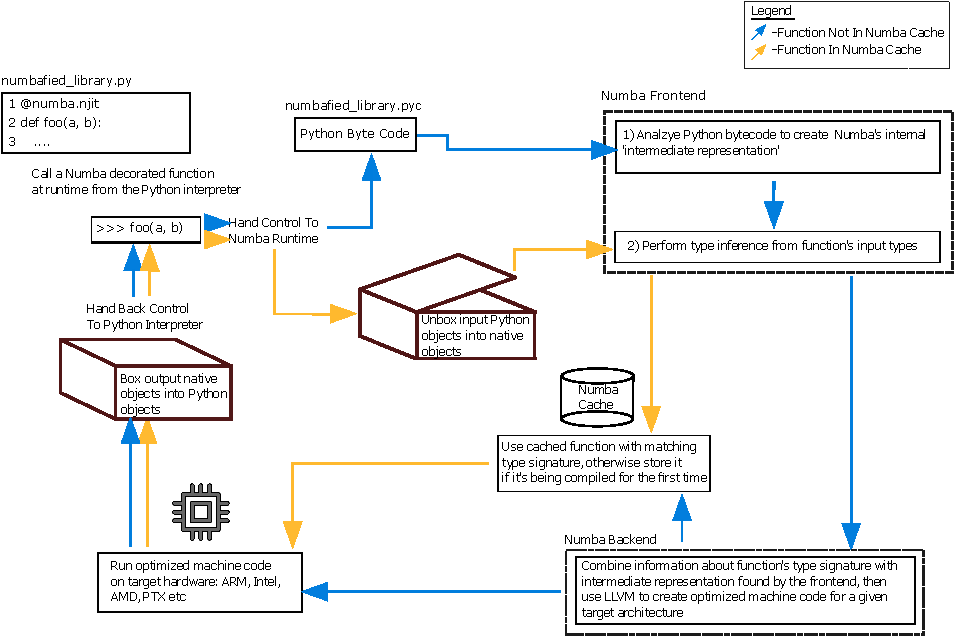
\includegraphics[width=\linewidth]{images/ch_1/numba.pdf}
    \caption{A visualisation of the Numba runtime system. A function decorated with `njit' acts as an instruction to the runtime to check a database for any Numba-compiled functions with a matching function signature, if this doesn't exist Numba generates a new compiled function and caches it using LLVM. Future calls of this function use this cached version in place of the Python interpreter. Code relies on Numba's runtime to correctly `box' and `unbox' native Python objects into data structures compatible with Numba code, which operates on a subset of numerical data structures created using the NumPy library.}
    \label{fig:chpt:1:sec:1:numba_runtime}
\end{figure}


